\subsection{Variational Auto-Encoders}

\subsubsection{Framework and optimization objective}

We are interested in another kind of latent models, this time based on variational inference
results to achieve a new kind of deep latent structure: the Variational Auto-Encoder (VAE).
These latent models were introduced in 2013 by Kingma, better described in a more in depth paper in 2019: see \cite{kingma2019introduction}

Once again, we assume the observations $X$ to be modelizable by a given distribution
parameterized by $\theta$:

$$
X \sim p_{\theta}(x)
$$

Determining $\theta$ holds to find one $\theta^*$ that would optimize a given objective, generally chosen as the maximum of likelihood. Indeed, if $\theta^* \in arg\max_{\theta} p_{\theta}(x)$, then such $\theta^*$ maximizes the density around the dense areas of the observations, which makes them highly likely to happen under such distribution $p_{\theta^*}$. Hence, the maximum likelihood is a natural criterion:
$$
\theta^* \in arg\max_{\theta} p_{\theta}(x)
$$

However, such modelization does not include a latent structure.
As a result, we try to enforce it by rewriting the objective as follows:

$$
p_{\theta}(x) = \int_{\mathcal{Z}} p(x,z) dz 
$$

Using Bayes decomposition, we obtain the following objective:
$$
p_{\theta}(x,z) = p_{\theta}(z) p_{\theta}(x|z)
$$

Recall that the prior $p_{\theta}(z)$ and the a priori $p_{\theta}(x|z)$ are defined by the framework (ex: Bernoulli prior and Gaussian posterior gives the Gaussian mixture framework). However, the computation of the evidence $p_{\theta}(x)$ is generally intractable in practice, which also leads to a non-tractable posterior distribution: $p_{\theta}(z|x)$. As a result, not being able to compute the evidence leads to not being able to provide a gradient regarding $\theta$, so we can not perform the backpropagation in a deep learning approach.

Note that there exist approximate inference techniques to compute the evidence and the
posterior, but these are quite expensive and often yield poor convergence results.

To overcome this issue, we introduce a smart rewriting of the objective using variational
inference.
Indeed, let $q_{\Phi}(z|x) \approx p_{\theta}(z|x)$ to be learnt over $\Phi$, one can write:
$$
\begin{align}
    \log p_{\theta}(x) &= \mathbb{E}_{q_{\Phi}(z|x)}[\log p_{\theta}(x)] \\
    &= \mathbb{E}_{q_{\Phi}(z|x)}\left[\log \frac{p_{\theta}(x)}{q_{\Phi}(z|x)} \frac{q_{\Phi}(z|x)}{p_{\theta}(z|x)}\right]
    \\
    &= \underbrace{\mathbb{E}_{q_{\Phi}(z|x)} \left[\log \frac{p_{\theta}(x)}{q_{\Phi}(z|x)}\right]}_{ELBO(q_\phi(z|x), p_{\theta}(x,z))} + D_{KL}\left[q_{\Phi}(z|x) \Vert p_{\theta}(z|x)\right]
\end{align}
$$

The first term of that decomposition is generally called the Evidence Lower BOund (ELBO),
as it marks a lower bound to the evidence $\log p_{\theta}(x)$ since the KL divergence is a
positive quantity:
$$
\log p_{\theta}(x) \ge ELBO(q_\phi(z|x), p_{\theta}(x,z))
$$

$q_{\Phi}(z|x)$ is an approximation of the true posterior $p_{\theta}(z|x)$ that we aim at
learning in a family of distributions. For instance,
$$
q_{\Phi}(.|x) \sim \mathcal{N}(\mu(x), \Sigma(x))
$$ 
would be an approximation of the true posterior by a Gaussian distribution.
Notice that the true posterior may very not likely be Gaussian, which creates a first
complexity error in our model.

Despite being a lower bound on the true maximum likelihood objective, the ELBO is actually tractable. Indeed, as we continue the computation:
$$
\begin{align}
    ELBO(q_\phi(z|x), p_{\theta}(x,z)) &= \mathbb{E}_{q_{\Phi}(z|x)}[\log p_{\theta}(x,z)] - \mathbb{E}_{q_{\Phi}(z|x)}[\log q_{\Phi}(z|x)] \\
    &= 
\mathbb{E}_{q_{\Phi}(z|x)}[\log p_{\theta}(x|z)] - D_{KL}[\log q_{\Phi}(z|x) \Vert p_{\theta}(z)] \\\end{align}
$$

Another remarkable fact, is that when maximizing the ELBO, we are actually minimizing the KL divergence between the estimated and the true posterior.
Hence, one can define the ELBO as a suboptimal objective to our problem that we get to maximize to obtain $(\Phi^*, \theta^*)$, the parameters of our model.

\subsubsection{Reparameterization trick}

Even though the gradient of the ELBO is well defined for $\theta$, it is not possible to compute the differential relatively to $\Phi$ yet, as it requires samples from the approximation to the posterior $q_{\Phi}(z|x)$ to compute $\mathbb{E}_{q_{\Phi}(z|x)}[\log p_{\theta}(x|z)]$.
\medskip

Since, sampling is not a differentiable operation, we make use of the change of variable formula, so that for a bijective transformation $z = \phi_x(\epsilon)$, we get:
$$
p(z) = p(\epsilon) \det \left| \frac{\partial \epsilon}{\partial z}\right|
$$

Hence, if we take $\epsilon$ a random variable of density $p(\epsilon)$ that does not depend on $\theta$, $\Phi$ nor $x$, so that $z = \phi_x(\epsilon)$, for any $L_1$ function $f$,
$$
\mathbb{E}_{q_{\Phi}(z|x)}[f(z)] = \mathbb{E}_{p(\epsilon)}[f(z)]
$$

As a result, the samples are not obtained through $q_{\Phi}$ anymore but through $p(\epsilon)$, so that can safely perform derivation of the ELBO relatively to $\Phi$ and backpropagate our gradient through the network.

\subsubsection{Architecture}

The vanilla architecture of the VAE is described by the following illustration:

\begin{figure}[H]
    \centering
    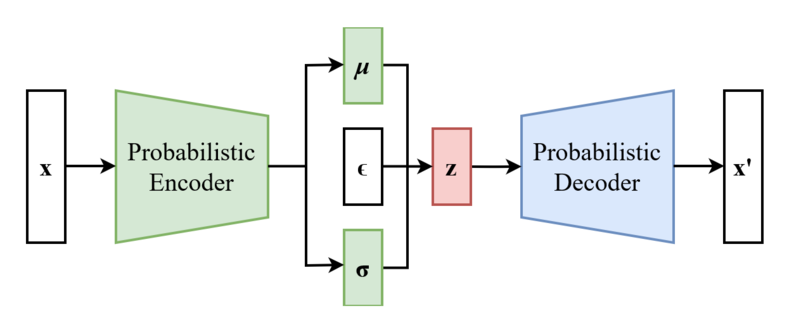
\includegraphics[width=.7\textwidth]{images/Reparameterized_Variational_Autoencoder}
    \caption{Illustration of a VAE with Gaussian prior (wikipedia)}
    \label{fig:vae_architecture}
\end{figure}

The first part is generally called the encoder, as it turns a sample $x$ into its latent representation $z$ by modelizing the posterior $q_{\Phi}(z|x)$. The second part is then called the decoder, as it throws a latent representation in the sample space. The latest can even serve as a generative architecture, as one can sample from the latent space through $q_{\Phi}(z|x)$, and decode it to obtain a new sample.
\medskip

As we can see more clearly in that illustration, we can see that $\Phi$ and $\theta$ are trained jointly through the ELBO, both serving for one part of the VAE at a time.
\medskip

The training procedure is straightforward: the entry is a sample $x$ and the output objective is the same sample $x$. We aim at train the VAE for learning the data space and its latent representation by learning how to reconstruct the samples through it.

\subsubsection{Limits for our problem}

As we have seen through the reparameterization trick, training a VAE architecture requires to be able to backpropagate
the gradient of the ELBO at each step.
We namely had to perform the reparameterization trick to circumvent the randomness operation which is not differentiable.
As a result, learning a discrete posterior is not possible with such architecture, since we would have to perform a projection
of the output of the encoder on a discrete space, which is not a differentiable operation.
\medskip

Yet, learning discrete representation of our data seems much more natural than continuous latent ones.
As we tend to categorize things as much as we can, describing behaviors with words for instance.
Furthermore, a discrete representation facilitates the interpretation of the latent space by ordering data distribution in simple bins.
\medskip

The next architecture, called the VQ-VAE, stands as a first fork option to the VAE with discrete posterior.


